\chapter{Realizzazioni sperimentali e valutazione}
\label{ProveSperimentali}
\thispagestyle{empty}

\vspace{0.5cm}

\noindent In questo capitolo illustriamo come sono stati condotti gli esperimenti per la valutazione del nostro algoritmo di tampering detection.
La prima parte \`e dedicata alla descrizione dei dataset utilizzati come riferimento, mostrando quali sistemi di acquisizione sono stati utilizzati e quali sono le metriche che abbiamo tenuto in considerazione.
Nella seconda parte, invece, entriamo nel dettaglio su quali sono stati i risultati a valle di tutta l'analisi sperimentale. 
\section{Acquisizione dei dataset}
Durante lo svolgimento della tesi abbiamo realizzato alcuni sistemi di acquisizione, in modo da avere un insieme di dataset (\textit{benchmark}) molto ampio che comprendesse sequenze video con diverse qualit\`a dei frame e con diversi framerate.
Alcune di queste sequenze sono state utilizzate per testare l'algoritmo di segmentazione, mentre altre hanno verificato l'algoritmo di tampering detection.
In generale, per ogni scena ripresa (dove per scena intendiamo una specifica inquadratura che \textit{non cambia} per le varie sequenze) abbiamo:
\begin{itemize}
	\item almeno una sequenza in cui non avviene nessun evento di tampering, che viene utilizzata per la creazione della mappa;
	\item almeno una sequenza in cui la camera subisce una sfocatura;
	\item almeno una sequenza in cui la camera subisce uno spostamento.
\end{itemize}
\subsection{Sistemi di acquisizione utilizzati}
\subsubsection{Camere ST}

\subsubsection{Raspberry Pi Camera}
Il sistema di acquisizione realizzato con le camere di ST aveva il problema di dover essere alimentato dalla rete elettrica.
Non \`e stato possibile, quindi, utilizzarlo per acquisizioni all'esterno.\\
Per ovviare a questo problema abbiamo deciso di realizzare un altro sistema basato su un \textit{Raspberry Pi modello B+} \cite{raspberry} con relativo \textit{modulo camera} \cite{raspberryCamera}.
Il Raspberry Pi (Fig. \ref{fig:raspberry}) \`e un \textit{single-board computer} (ovvero un computer implementato su una singola scheda elettronica) basato su un \textit{system-on-chip} (SoC) \textit{Broadcom BCM2835} \cite{broadcom}, che incorpora un processore \textit{ARM1176JZF-S} \cite{arm}, una GPU \textit{VideoCore IV} \cite{gpu} e $512$ MB di memoria.
Utilizza un sistema operativo \textit{Debian Linux} realizzato per processori ARM chiamato \textit{Raspbian} \cite{raspbian}.
Le ridotte dimensioni e il basso consumo di potenza hanno permesso l'utilizzo del Raspberry Pi per fare le acquisizioni in ambienti esterni, utilizzando una batteria per alimentare il tutto. 
\begin{figure}
	\centering
	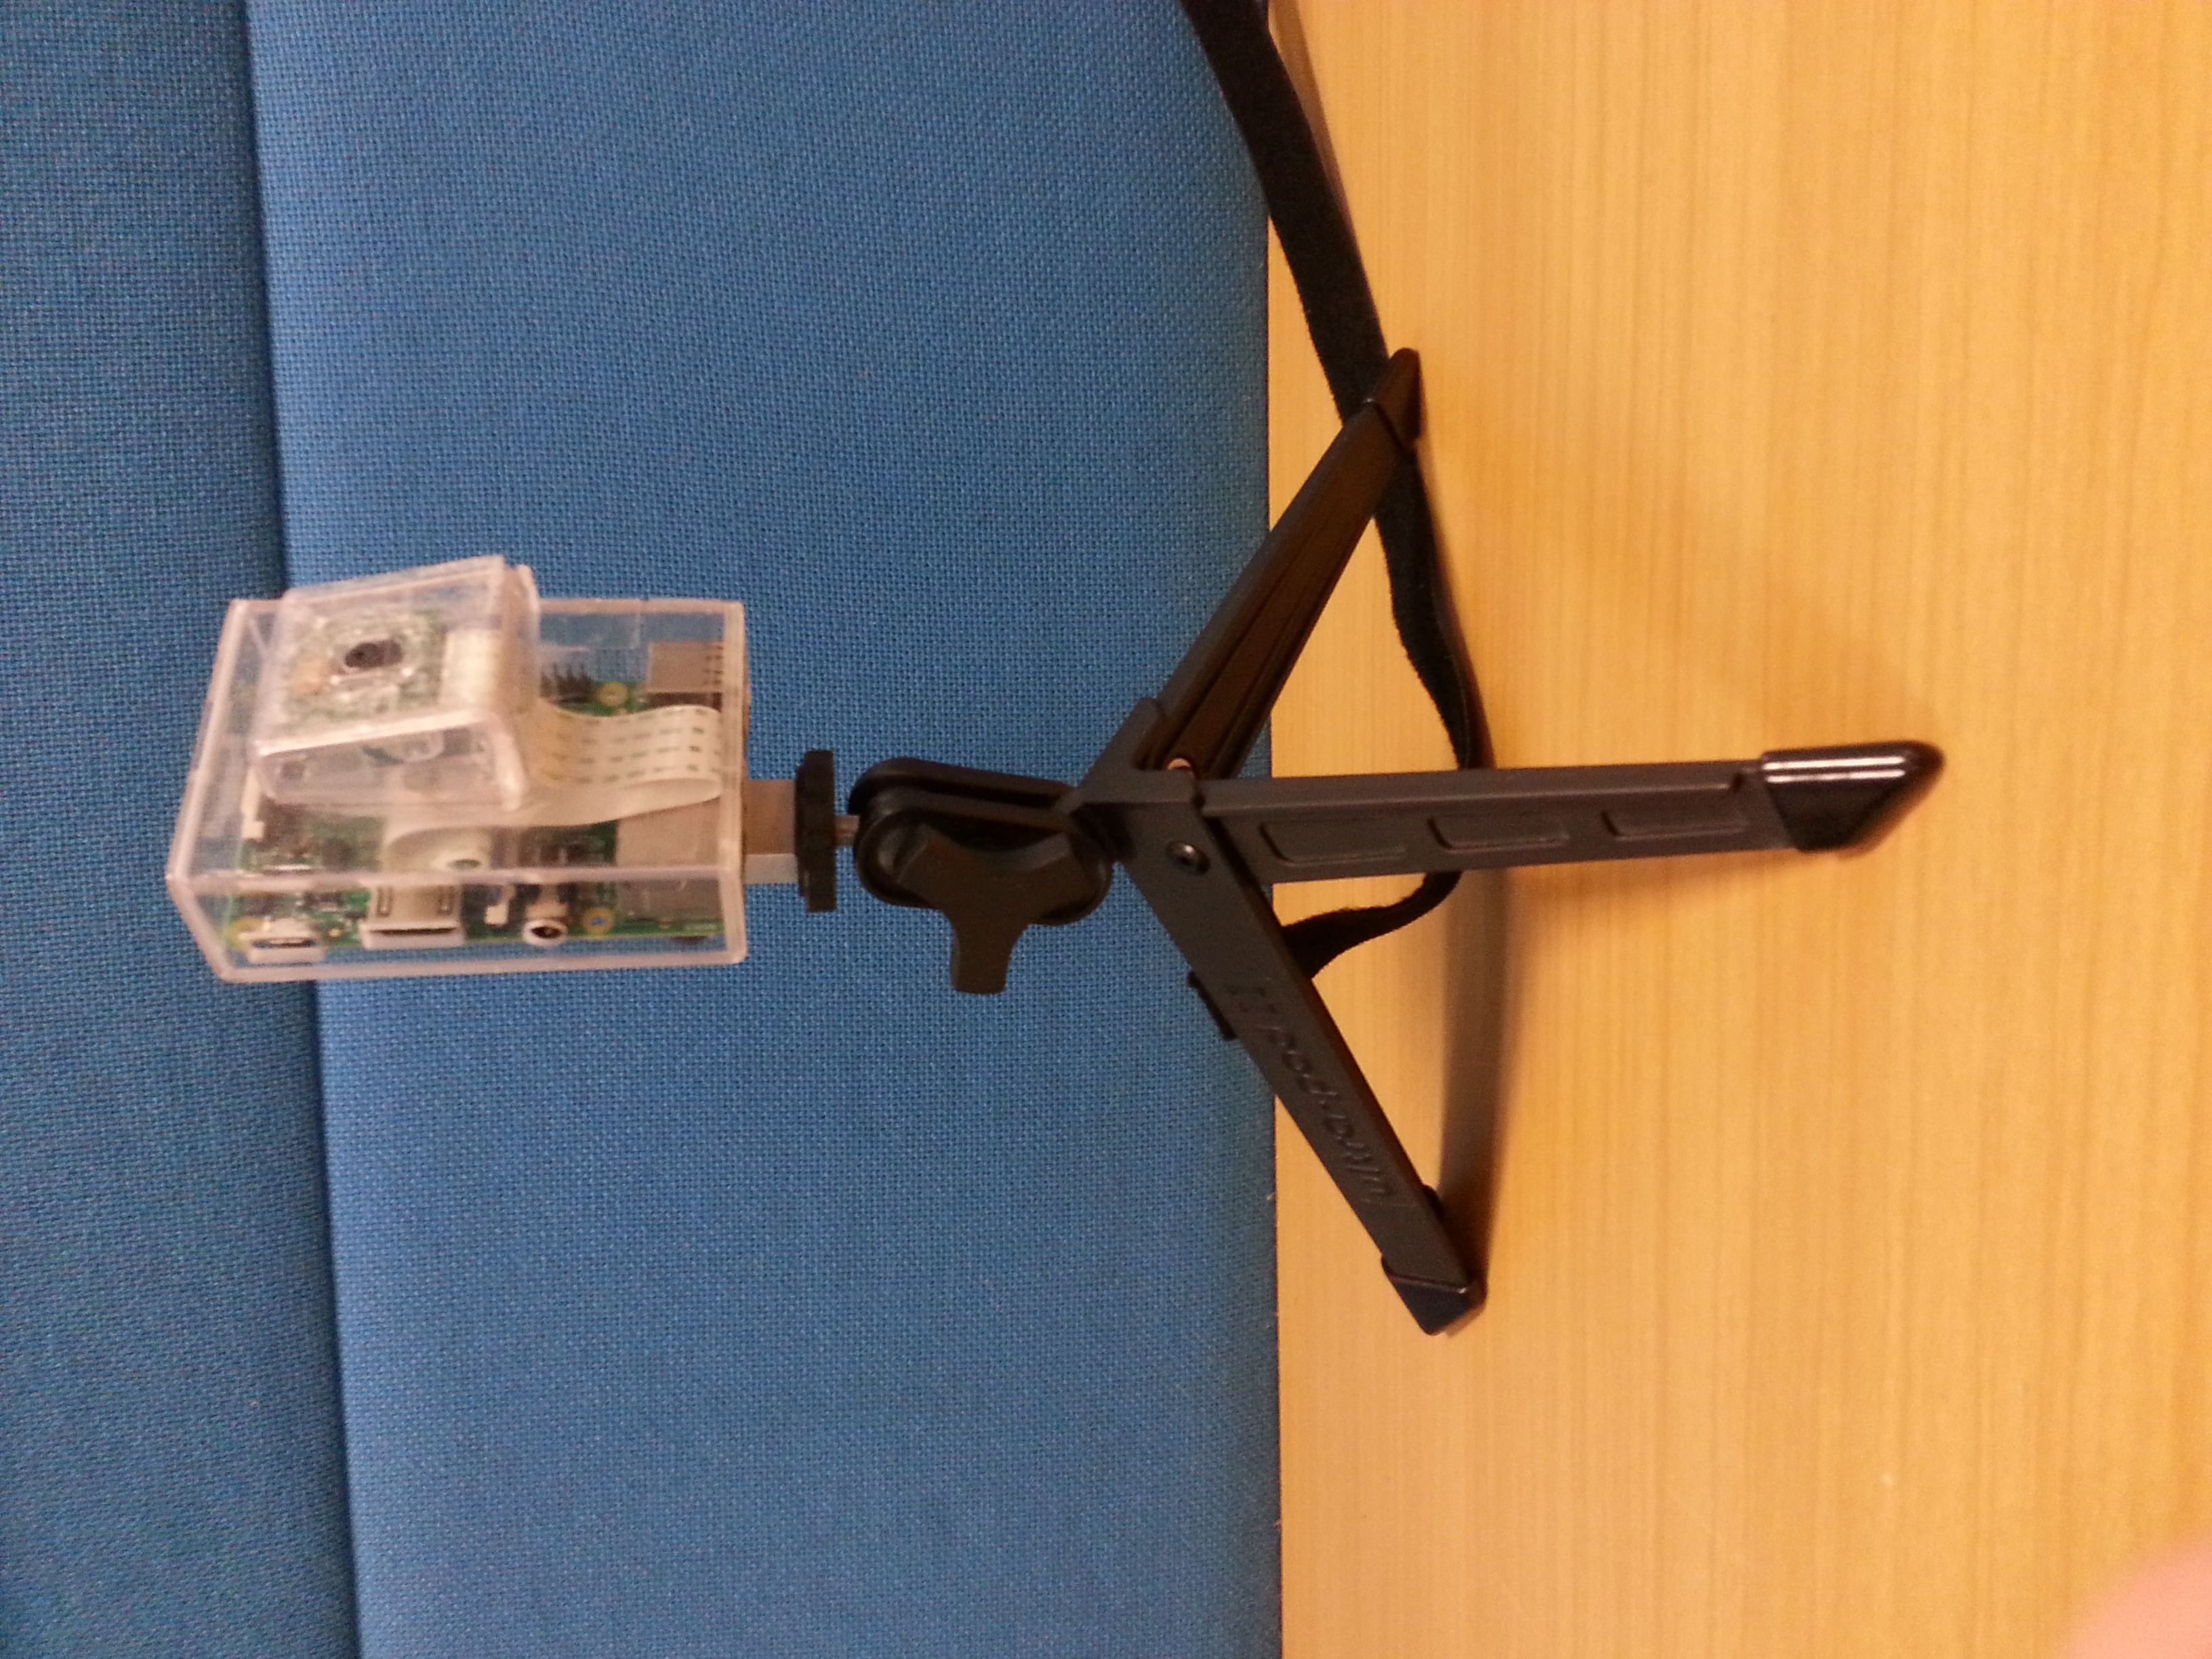
\includegraphics[width=6cm]{./pictures/raspberry}
	\caption{Il Raspberry Pi utilizzato per l'acquisizione}
	\label{fig:raspberry}
\end{figure}
Per interfacciarci con il dispositivo abbiamo creato una \textit{connessione SSH}, tramite USB, con uno smartphone: in questo modo abbiamo potuto lanciare i comandi necessari per far partire l'acquisizione. 
% FARE UNA FOTO DI RASPBERRY CON CELLULARE CON SU SSH
Per l'acquisizione abbiamo creato uno script in \textit{Python}, utilizzando la libreria \textit{picamera} \cite{picamera} per interfacciarci con il modulo camera.
%METTERE SCRIPT UTILIZZATO PER L'ACQUISIZIONE
\subsubsection{Estrazione frame dal web}
Un ultimo dataset \`e stato generato utilizzando sequenze di frame presenti sul portale di previsioni del tempo \textit{ilMeteo.it} \cite{ilmeteo}, 
\subsection{Sequenze con presenza di tampering}
\subsection{Definizione dei ground thruth}
\subsection{Definizione delle metriche per la stima delle prestazioni}
\section{Risultati ottenuti}